\documentclass[11pt]{article}
\usepackage[a4paper,margin=1in]{geometry}
\usepackage{amsmath,amssymb,amsthm}
\usepackage{tikz}
\usepackage{booktabs}
\usepackage{xcolor}
\usepackage[hidelinks]{hyperref}
\hypersetup{pdftitle={Why the sphere beats the ball},pdfauthor={Vamshi Jandhyala}}
\setlength{\parskip}{0.4em}
\setlength{\parindent}{0pt}

\newtheorem{theorem}{Theorem}
\newtheorem{corollary}{Corollary}
\newtheorem{lemma}{Lemma}
\newtheorem{proposition}{Proposition}
\theoremstyle{remark}
\newtheorem*{remark}{Remark}

\definecolor{inkblue}{RGB}{40,76,105}
\definecolor{softblue}{RGB}{226,235,243}
\definecolor{rust}{RGB}{153,70,45}

\title{Why the sphere beats the ball}
\author{Vamshi Jandhyala}
\date{}

\begin{document}
\maketitle
\vspace{-2em}

\begin{abstract}
Three random points on a circle form an acute triangle less often than three random points in the disc, but
three random points on a sphere do so more often than three in the ball. We explain the second half exactly.
For three points with independent uniform directions on concentric spheres of radii $a\ge b\ge c>0$ we find the
probability of an acute triangle in closed form and show that it is at most $\frac12$, with equality only when
the two largest radii are equal. Consequently the uniform sphere is the unique best rotationally invariant
distribution in space, and the ball must lose to it. In the plane, by a recent result of Greenwell, the best
such law instead puts a vertex at the centre, and a small amount of mass at the centre helps the circle; this
is where the two dimensions part ways. The algebra and the integrals are checked in the Lean
proof assistant.
\end{abstract}

\section{The question}

Choose three independent uniform points from a set and ask how often they form an acute triangle. Dan asked on
MathOverflow~\cite{MO} why the four classical answers behave as they do:
\begin{center}
\begin{tabular}{lcc}
\toprule
 & boundary & interior \\
\midrule
plane & circle: $\frac14$ & disc: $\frac4{\pi^2}-\frac18\approx0.280$ \\
space & sphere: $\frac12$ & ball: $\frac{33}{70}\approx0.471$ \\
\bottomrule
\end{tabular}
\end{center}
The disc and ball values are Hall's~\cite{Hal82}; the circle value is classical. Filling in the circle helps, but
filling in the sphere hurts. Here is a version to try before reading on. Three points on a sphere give an acute
triangle half the time. Now pull one of them inside, to a smaller sphere with the same centre, keeping its
direction uniform. Does the chance go up or down?

It goes down, and the same happens whatever the three radii are, unless the two largest agree.

\begin{theorem}\label{thm:main}
Let $A,B,C$ be independent, uniform on the spheres of radii $a\ge b\ge c>0$ centred at the origin of
$\mathbb R^3$, and put $h=\sqrt{\max(0,\,b^2+c^2-a^2)}$. Then
\[
P(a,b,c)=\Pr(ABC\text{ is acute})=\frac b{2a}+\frac{c^2}{6ab}-\frac{h^3}{6abc}\;\le\;\frac12 ,
\]
with equality if and only if $a=b$.
\end{theorem}

Read the formula with $a=b=c$: then $h=c$ and $P=\frac12+\frac16-\frac16$, the sphere. Moving the outer point
further out ($a$ larger) costs at once (Figure~\ref{fig:curves}, left), and moving the inner point in costs
nothing only while the other two share a sphere.

\begin{corollary}\label{cor:law}
Let $X,Y,Z$ be independent with a common rotationally invariant distribution on $\mathbb R^3$. Then
$\Pr(XYZ\text{ is acute})\le\frac12$, with equality if and only if the distribution is uniform on a sphere
centred at the origin. In particular the ball, whose radius is spread out, does worse than the sphere, whatever
its exact value.
\end{corollary}

The plane behaves differently. Greenwell~\cite{Gre26} recently solved the planar version of
Theorem~\ref{thm:main}, three concentric circles, and showed that there too the acute probability is at most
$\frac12$ for every rotationally symmetric law; but in the plane equality needs one vertex at the centre and the
other two on a common circle, so the uniform circle, at $\frac14$, is far from the best. In space the sphere is the
best. That is the asymmetry the question asks about, and a two-line experiment shows it
(Section~\ref{sec:plane}): put a small mass $\varepsilon$ at the centre and the probability rises for the circle
but falls for the sphere (Figure~\ref{fig:curves}, right). Greenwell notes that the fixed-radius formula for
spheres was not known; Theorem~\ref{thm:main} supplies it in $\mathbb R^3$. What we do not have is a direct proof
that the disc's particular spread helps; its value is only known by computing it.

\begin{figure}[ht]
\centering
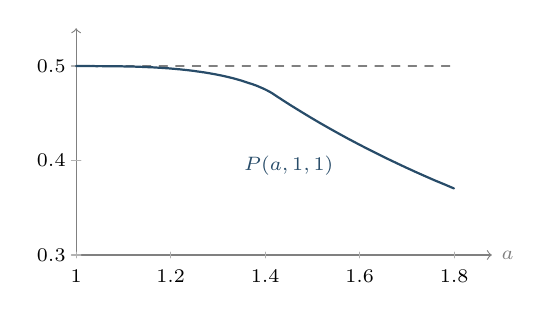
\begin{tikzpicture}[x=6cm,y=12cm,line cap=round]
  % left: P(a,1,1) for a from 1 to 1.8
  \draw[->,gray] (1,0.3) -- (1.88,0.3) node[right,font=\scriptsize] {$a$};
  \draw[->,gray] (1,0.3) -- (1,0.54);
  \foreach \y in {0.3,0.4,0.5} \draw[gray!60] (0.99,\y) -- (1.01,\y) node[left=2pt,font=\scriptsize,black] {$\y$};
  \foreach \x in {1,1.2,1.4,1.6,1.8} \draw[gray!60] (\x,0.297) -- (\x,0.303) node[below=3pt,font=\scriptsize,black] {$\x$};
  \draw[gray,dashed] (1,0.5) -- (1.8,0.5);
  \draw[inkblue,thick,domain=1:1.4142,samples=80] plot (\x,{1/(2*\x)+1/(6*\x)-(2-\x*\x)^(1.5)/(6*\x)});
  \draw[inkblue,thick,domain=1.4142:1.8,samples=20] plot (\x,{1/(2*\x)+1/(6*\x)});
  \node[font=\scriptsize,inkblue] at (1.45,0.395) {$P(a,1,1)$};
\end{tikzpicture}
\hspace{1.5em}
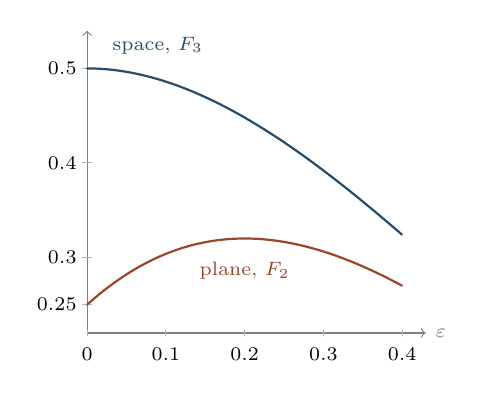
\begin{tikzpicture}[x=10cm,y=12cm,line cap=round]
  \draw[->,gray] (0,0.22) -- (0.43,0.22) node[right,font=\scriptsize] {$\varepsilon$};
  \draw[->,gray] (0,0.22) -- (0,0.54);
  \foreach \y in {0.25,0.3,0.4,0.5} \draw[gray!60] (-0.006,\y) -- (0.006,\y) node[left=2pt,font=\scriptsize,black] {$\y$};
  \foreach \x in {0,0.1,0.2,0.3,0.4} \draw[gray!60] (\x,0.217) -- (\x,0.223) node[below=3pt,font=\scriptsize,black] {$\x$};
  \draw[rust,thick,domain=0:0.4,samples=60] plot (\x,{(1-\x)^2*(1+5*\x)/4});
  \draw[inkblue,thick,domain=0:0.4,samples=60] plot (\x,{(1-\x)^2*(1+2*\x)/2});
  \node[font=\scriptsize,inkblue,anchor=south west] at (0.02,0.505) {space, $F_3$};
  \node[font=\scriptsize,rust,anchor=north] at (0.2,0.305) {plane, $F_2$};
\end{tikzpicture}

\caption{Left: $P(a,1,1)$ from Theorem~\ref{thm:main}, one point on a sphere of radius $a\ge1$ and two on the unit
sphere; it starts at $\frac12$ and falls. Right: the centre experiment of Section~\ref{sec:plane}, a point at the
centre with probability $\varepsilon$, otherwise uniform on the circle or sphere.}
\label{fig:curves}
\end{figure}

\section{Caps on a sphere}

Everything reduces to one-dimensional integrals because of Archimedes' hat-box theorem: if $W$ is uniform on a
sphere of radius $w$ in $\mathbb R^3$, its projection onto any fixed line through the centre is uniform on
$[-w,w]$.

\begin{lemma}\label{lem:obtuse}
The angle of triangle $UVW$ at $W$ is obtuse if and only if $(U+V)\cdot W>U\cdot V+|W|^2$.
\end{lemma}

\begin{proof}
The angle at $W$ is obtuse when $(U-W)\cdot(V-W)<0$, and expanding gives
$U\cdot V-(U+V)\cdot W+|W|^2<0$.
\end{proof}

So once $U$ and $V$ are fixed, the bad positions of $W$ form a cap: the part of its sphere beyond a plane
perpendicular to $U+V$ (Figure~\ref{fig:cap}).

\begin{figure}[ht]
\centering
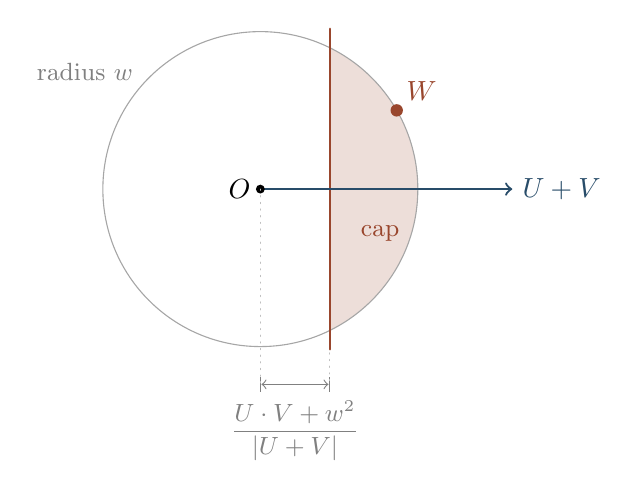
\begin{tikzpicture}[scale=1.6,line cap=round]
  % cross-section: the sphere of radius w carrying W, the direction of U+V, and the cap where the angle at W is obtuse
  \def\w{1.25}
  \def\t{0.55}
  \fill[rust!18] (\t,{sqrt(\w*\w-\t*\t)}) arc ({acos(\t/\w)}:{-acos(\t/\w)}:\w) -- cycle;
  \draw[gray!70] (0,0) circle (\w);
  \draw[rust,thick] (\t,{-sqrt(\w*\w-\t*\t)-0.15}) -- (\t,{sqrt(\w*\w-\t*\t)+0.15});
  \draw[->,inkblue,thick] (0,0) -- (2.0,0) node[right] {$U+V$};
  \fill (0,0) circle (1pt) node[left] {$O$};
  \draw[|<->|,gray] (0,-1.55) -- (\t,-1.55);
  \node[font=\small,gray,anchor=north] at (\t/2,-1.6) {$\dfrac{U\cdot V+w^2}{|U+V|}$};
  \draw[gray!50,dotted] (0,0) -- (0,-1.55);
  \draw[gray!50,dotted] (\t,-1.3) -- (\t,-1.55);
  \node[rust,font=\small] at (0.95,-0.35) {cap};
  \node[font=\small,gray,anchor=east] at ({-\w*cos(45)-0.05},{\w*sin(45)+0.05}) {radius $w$};
  \fill[rust] ({\w*cos(30)},{\w*sin(30)}) circle (1.4pt) node[above right] {$W$};
\end{tikzpicture}

\caption{With $U$ and $V$ fixed, the angle at $W$ is obtuse exactly when $W$ lies in the shaded cap, beyond the
plane at height $(U\cdot V+w^2)/|U+V|$ along $U+V$.}
\label{fig:cap}
\end{figure}

Let $u,v,w$ be the radii of $U,V,W$ and $M=|U+V|$. By the hat-box theorem $U\cdot V/(uv)$ is uniform on
$[-1,1]$, so from $M^2=u^2+v^2+2U\cdot V$ the length $M$ has density $M/(2uv)$ on $[|u-v|,u+v]$. Given $U$ and
$V$, the projection $(U+V)\cdot W$ is uniform on $[-wM,wM]$, so it exceeds the threshold $T=U\cdot
V+w^2=\frac12(M^2+w^2-K)$, with $K=u^2+v^2-w^2$, with probability $(wM-T)/(2wM)$ clipped to $[0,1]$.
Simplifying, $(wM-T)/(2wM)=\bigl(K-(M-w)^2\bigr)/(4wM)$, and the probability of an obtuse angle at $W$ is
\begin{equation}\label{eq:pw}
p_W=\int_{|u-v|}^{u+v}\max\Bigl(0,\;\min\Bigl(\frac M{2uv},\;\frac{K-(M-w)^2}{8uvw}\Bigr)\Bigr)\,dM .
\end{equation}
Read the integrand as: the density of $M$, times the fraction of $W$'s sphere in the cap. The $\min$ is the
case of a full cap ($W$ is always bad), the $\max$ the case of an empty one.

\section{The three angles}

Order the radii $a\ge b\ge c>0$. In each of the three integrals~\eqref{eq:pw} the clipping happens at simple
places, and what is left is a polynomial in $M$.

\emph{The smallest radius, $W=C$.} Here $K=a^2+b^2-c^2$; write $H=\sqrt K$. The cap is full for $M\le H-c$,
partial for $H-c\le M\le H+c$, and empty beyond. These points lie in $[a-b,a+b]$, because
$K-(a-b+c)^2=2(a+c)(b-c)\ge0$ and $(a+b-c)^2-K=2(a-c)(b-c)\ge0$. Integrating the two polynomial pieces,
\[
p_C=\frac{(H-c)^2-(a-b)^2}{4ab}+\frac{2cK-\frac13\bigl(H^3-(H-2c)^3\bigr)}{8abc}=\frac12-\frac{c^2}{3ab}.
\]

\emph{The middle radius, $W=B$.} Here $K=a^2+c^2-b^2$ and the cap is partial on the whole range $[a-c,a+c]$:
the numerator $K-(M-b)^2$ is a concave quadratic in $M$ and is nonnegative at both ends, where it equals
$2(a-b)(b+c)$ and $2(a-b)(b-c)$, and the full-cap condition $M+b\le\sqrt K$ fails since
$(a-c+b)^2-K=2(a+b)(b-c)\ge0$. So
\[
p_B=\int_{a-c}^{a+c}\frac{K-(M-b)^2}{8abc}\,dM=\frac{a-b}{2a}+\frac{c^2}{6ab}.
\]

\emph{The largest radius, $W=A$.} Here $K=b^2+c^2-a^2$. If $K\le0$ the cap is always empty and $p_A=0$.
Otherwise $h=\sqrt K\le c$, the cap is partial for $|M-a|<h$ and empty elsewhere, and
$[a-h,a+h]\subseteq[b-c,b+c]$ because $(a-b+c)^2-h^2=2(a+c)(a-b)\ge0$ and $(b+c-a)^2-h^2=2(a-b)(a-c)\ge0$. So
\[
p_A=\int_{a-h}^{a+h}\frac{h^2-(M-a)^2}{8abc}\,dM=\frac{h^3}{6abc},
\]
which is also right when $K\le0$, with $h=0$.

A triangle has at most one obtuse angle, and a right angle has probability zero, so
$P=1-p_A-p_B-p_C$, which is the formula of Theorem~\ref{thm:main}.

\section{The bound}

\begin{proof}[Proof of Theorem~\ref{thm:main}]
Fix $b\ge c>0$ and let the largest radius $a$ grow from $b$. Put
\[
G(a)=6abc\Bigl(\frac12-P\Bigr)=3bc(a-b)-c^3+h^3 .
\]
At $a=b$ we have $h=c$ and $G(b)=0$. While $b^2+c^2>a^2$, $h^3=(b^2+c^2-a^2)^{3/2}$ and
\[
G'(a)=3(bc-ah),\qquad b^2c^2-a^2h^2=b^2c^2-a^2(b^2+c^2-a^2)=(a^2-b^2)(a^2-c^2),
\]
which is positive for $a>b$; so $G$ is strictly increasing there. Once $a^2\ge b^2+c^2$, $h=0$ and $G$ grows
linearly with slope $3bc$. Hence $G(a)>0$ for $a>b$: $P<\frac12$ unless $a=b$, and $P=\frac12$ when $a=b$.
\end{proof}

\begin{proof}[Proof of Corollary~\ref{cor:law}]
A rotationally invariant random point is $R\Theta$ with $\Theta$ uniform on the unit sphere and independent of
the radius $R\ge0$. Condition on the three radii. If all are positive, Theorem~\ref{thm:main} gives at most
$\frac12$. If exactly one is $0$, say the triangle is $OA'B'$ with $|A'|=a\ge|B'|=b>0$, then it is acute exactly
when $0<A'\cdot B'<b^2$, which has probability $b/(2a)\le\frac12$ because $A'\cdot B'/(ab)$ is uniform on
$[-1,1]$. If two are $0$ the triangle is degenerate. So the probability is at most $\frac12$. Equality needs
equality almost surely in every case. If $R$ is not almost surely one positive constant, choose a level $r$
with $\Pr(R>r)$ and $\Pr(R\le r)$ both positive; with positive probability exactly one of the three radii exceeds
$r$, so the largest radius is unique and the conditional probability is below $\frac12$ (or, with two radii at
$0$, it is $0$).
\end{proof}

\begin{remark}
Theorem~\ref{thm:main} also gives the ball's value independently of Hall: with radial density $3r^2$, scale the
largest of the three radii to $1$, so the other two have joint density $18b^2c^2$ on $0<c<b<1$; integrating the
formula gives $\frac{18}{35}-\frac3{70}=\frac{33}{70}$.
\end{remark}

\section{The plane is different}\label{sec:plane}

Put one vertex at the centre $O$ and two uniform on the circle or sphere. The angles at the two boundary points
are acute, since $(O-U)\cdot(V-U)=1-U\cdot V>0$, and the angle at $O$ is acute exactly when $U\cdot V>0$, which
has probability $\frac12$ by the symmetry $V\mapsto-V$. So this triangle is acute half the time in either
dimension. Now let each point be the centre with probability $\varepsilon$ and uniform on the boundary
otherwise. No centre gives the boundary value, one centre gives $\frac12$, and two or three give a degenerate
triangle:
\begin{align*}
F_2(\varepsilon)&=\frac{(1-\varepsilon)^3}4+\frac{3\varepsilon(1-\varepsilon)^2}2=\frac{(1-\varepsilon)^2(1+5\varepsilon)}4
&&\text{(plane)},\\
F_3(\varepsilon)&=\frac{(1-\varepsilon)^3}2+\frac{3\varepsilon(1-\varepsilon)^2}2=\frac{(1-\varepsilon)^2(1+2\varepsilon)}2
&&\text{(space)}.
\end{align*}
In the plane $F_2'(0)=\frac34>0$, and for example $F_2(\frac1{10})=\frac{243}{800}>\frac14$: the circle is not
even a local best. In space $F_3(\varepsilon)=\frac12-\frac32\varepsilon^2+\varepsilon^3<\frac12$ for
$0<\varepsilon\le1$, as Corollary~\ref{cor:law} requires. The difference is the boundary value: a triangle with a
vertex at the centre is acute half the time in both dimensions, which is better than the circle's $\frac14$ and
no better than the sphere's $\frac12$. By Greenwell's planar bound~\cite{Gre26}, a vertex at the centre with the
other two on one circle is in fact the best the plane can do.

\begin{remark}
This does not prove that the uniform disc beats the circle: the disc spreads its mass over all radii, not just
the centre, and very unequal radii can hurt in the plane too. A direct geometric reason for the disc's gain is
still missing. The wider question, which distribution in space maximises the probability without assuming
rotational invariance, is open; for uniform points in convex bodies Hall conjectured that the ball is best, and
Khan showed it is a local maximum~\cite{Hal82,Kha20}. Corollary~\ref{cor:law} answers the rotationally invariant
case of the question asked on Mathematics Stack Exchange~\cite{MSE}.
\end{remark}

\paragraph{Verification.} Lemma~\ref{lem:obtuse}, the clipped uniform tail and the form of the integrand
in~\eqref{eq:pw}, the three integrals $p_A,p_B,p_C$ for every $a\ge b\ge c>0$, the formula and the bound of
Theorem~\ref{thm:main} with its equality case, the one-centre case $b/(2a)\le\frac12$ and the two mixture
polynomials are checked in Lean~4 with Mathlib~\cite{mathlib}, using only the standard axioms. Quoted rather than
formalised: the hat-box theorem and the conditioning that turns it into~\eqref{eq:pw}, and the decomposition of
a rotationally invariant law used in the proof of Corollary~\ref{cor:law}. A Python program checks the three
cap probabilities against direct numerical integration of the defining integrals for 43 radius triples, and the
mixture and ball arithmetic exactly; six deliberately wrong variants fail it. An independent program, sharing no
code with it, estimates $P(a,b,c)$, the ball value and the mixtures by simulating actual points, and integrates
the formula exactly against the ball's radial density to get $\frac{33}{70}$. Everything is at
\url{https://github.com/jvvk/mathematics/tree/main/why-the-sphere-beats-the-ball}.

\paragraph{Acknowledgements.} Dan asked the question. Anthropic's Claude (Opus~5.5) was used to find the
argument, write the Lean formalisation and the programs, and draft this text. The author takes responsibility
for the content.

\begin{thebibliography}{9}
\bibitem{Gre26} B.~M.~Greenwell, Random triangles on concentric circles, arXiv:2608.06591 (2026).
\bibitem{Hal82} G.~R.~Hall, Acute triangles in the $n$-ball, \emph{J. Appl. Probab.} \textbf{19} (1982)
712--715, \href{https://doi.org/10.2307/3213533}{doi:10.2307/3213533}.
\bibitem{Kha20} G.~Khan, Hall's conjecture on extremal sets for random triangles, \emph{J. Geom. Anal.}
\textbf{30} (2020) 3413--3457, \href{https://doi.org/10.1007/s12220-019-00202-6}{doi:10.1007/s12220-019-00202-6}.
\bibitem{MO} Dan, Paradox involving probability that a triangle is acute in circles and spheres, MathOverflow
question 484567 (21 December 2024), \url{https://mathoverflow.net/q/484567}, accessed 10 October 2026.
\bibitem{MSE} Dan, What is the maximum probability that three random points, chosen from some set of points in
3D space, are the vertices of an acute triangle?, Mathematics Stack Exchange question 5012846 (18 December 2024),
\url{https://math.stackexchange.com/q/5012846}, accessed 10 October 2026.
\bibitem{mathlib} The mathlib Community, The Lean mathematical library, in \emph{Proceedings of the 9th ACM
SIGPLAN International Conference on Certified Programs and Proofs (CPP 2020)}, 367--381,
\href{https://doi.org/10.1145/3372885.3373824}{doi:10.1145/3372885.3373824}.
\end{thebibliography}

\bigskip
\noindent Vamshi Jandhyala, London, UK.

\end{document}
